\section{Cook}\label{sec:cook} % (fold)

Für die Reproduktion des Workflows mit identischer Einrichtung werden zwei Programme benötigt: nginx
als Reverse Proxy sowie Docker zur Ausführung des n8n-Containers, der Mongo-Datenbank und der
Einkaufslisten-App.

Im bereitgestellten ZIP-Archiv befindet sich die Datei \verb|n8n.conf|. In dieser Datei ist in Zeile 4
und in Zeile 13 der korrekte Domainname einzutragen. In Zeile 10 und in Zeile 11 sind der Pfad zum
SSL-Zertifikat und der Pfad zum zugehörigen privaten Schlüssel anzupassen. Nach der Anpassung wird
die Datei in das Verzeichnis \verb|/etc/nginx/sites-available| kopiert und mit einem aussagekräftigen
Namen, beispielsweise n8n, versehen. Anschließend wird im Verzeichnis
\verb|/etc/nginx/sites-enabled| ein
symbolischer Link auf die Konfigurationsdatei erstellt:

\begin{verbatim}
ln -s /etc/nginx/sites-available/n8n /etc/nginx/sites-enabled/n8n
\end{verbatim}

Dasselbe vorgehen muss mit der Datei \ver|shopping.conf| wiederholt werden.

Damit die Änderungen wirksam werden, ist der nginx-Dienst neu zu laden:

\begin{verbatim}
nginx -s reload
\end{verbatim}

Im entpackten ZIP-Archiv befindet sich ebenfalls die Datei \verb|.env.example|. Diese ist in
\verb|.env| umzubenennen. In der Datei wird der Domainname eingetragen. Der Start von n8n und
MongoDB erfolgt über den folgenden Befehl:

\begin{verbatim}
docker compose up
\end{verbatim}

Standardmäßig wird dabei die aktuelle stabile Version von n8n verwendet. Die gewünschte Version kann
in der Datei \verb|docker-compose.yml| festgelegt werden. Die zuletzt getestete Version ist
\verb|1.105.3|.

Beim ersten Aufruf des n8n-Servers wird die Erstellung eines Benutzerkontos abgefragt. Nach
erfolgreichem Abschluss der Registrierung erfolgt die Weiterleitung zur Übersichtsseite, die
\autoref{fig:n8n_overview} dargestellt ist.

\begin{figure}
    \begin{center}
        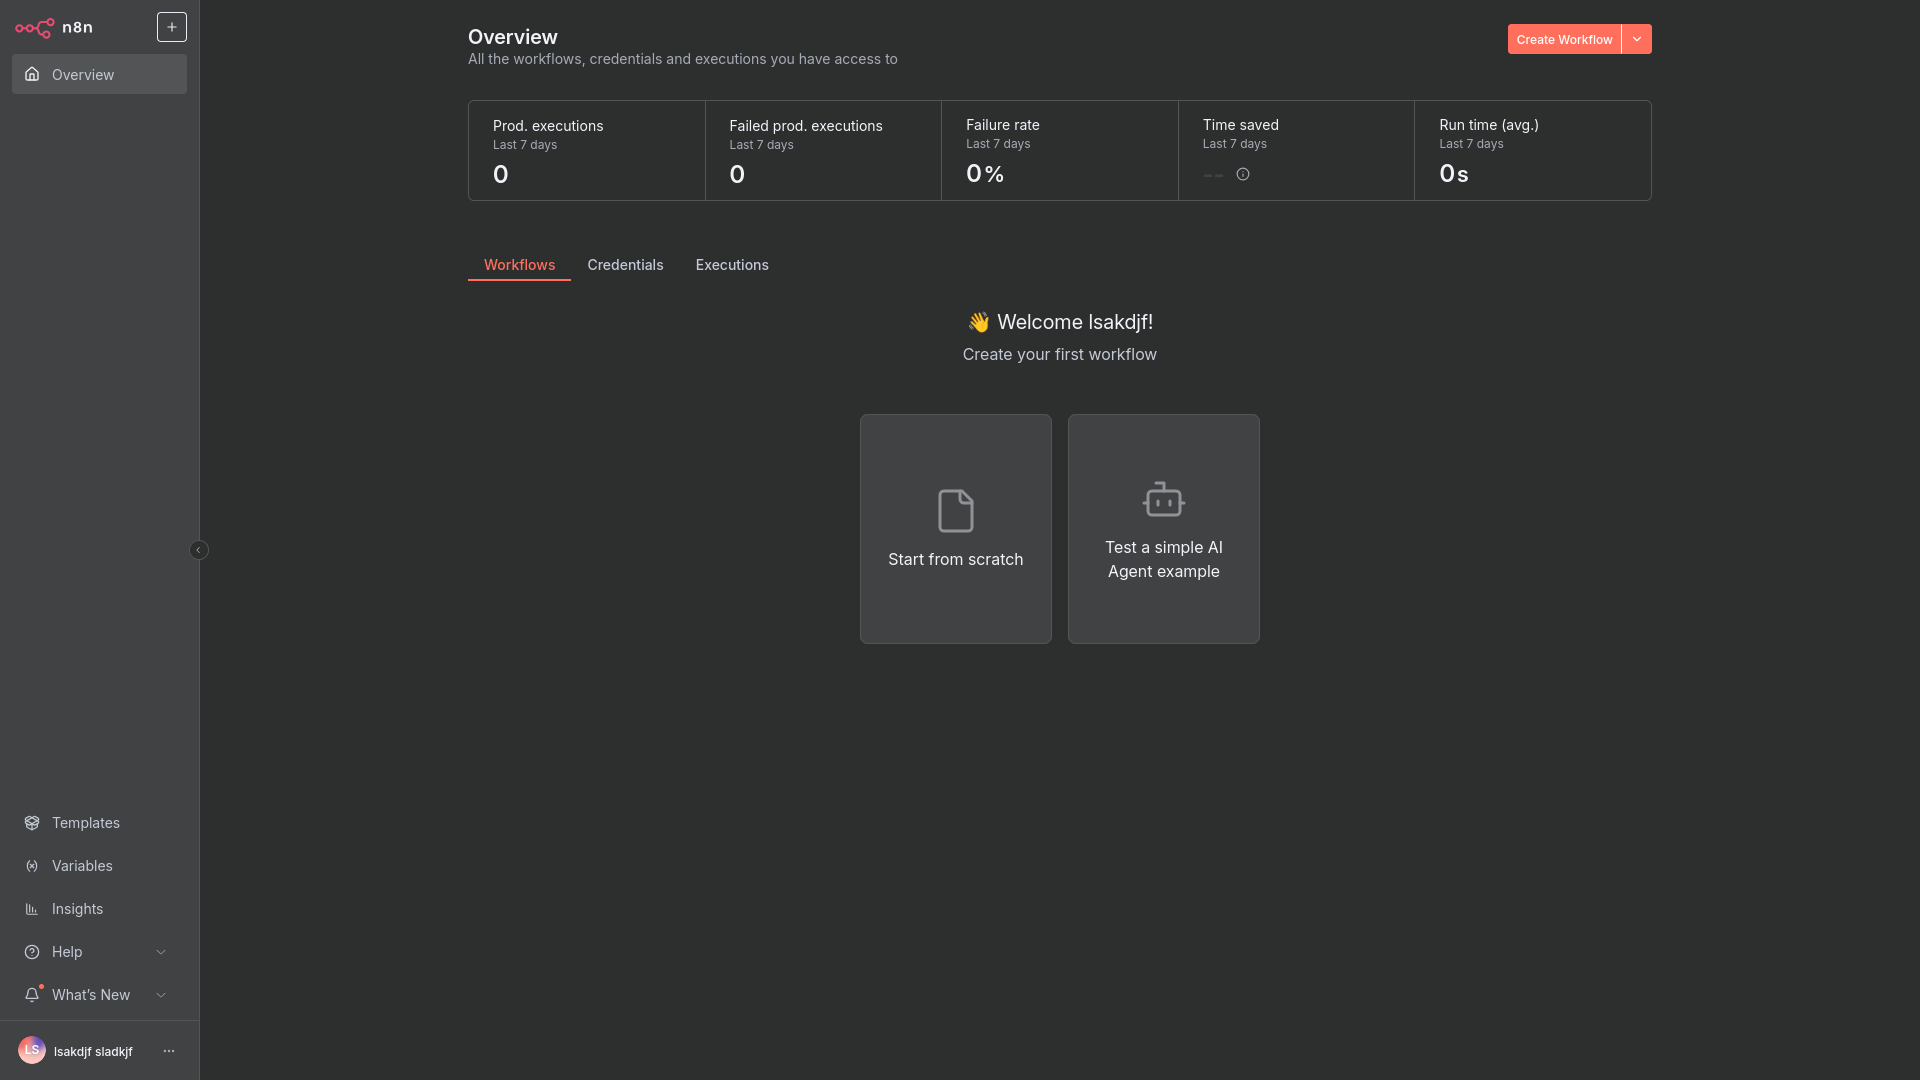
\includegraphics[width=0.95\textwidth]{images/n8n_overview.png}
    \end{center}
    \caption{n8n Übersichtsseite}\label{fig:n8n_overview}
\end{figure}

In n8n selber müssen zunächst im \enquote{Credentials} Reiter zwei Zugangsdaten angelegt werden. Für
die MongoDB muss in den Feldern \enquote{Database}, \enquote{User} und \enquote{Password} die Daten
eingetragen werden, die in der \verb|.env| Datei als \verb|MONGO_APP_DB|, \verb|MONGO_APP_USER| und
\verb|MONGO_APP_PASS| festgelegt wurden.

\begin{figure}
    \begin{center}
        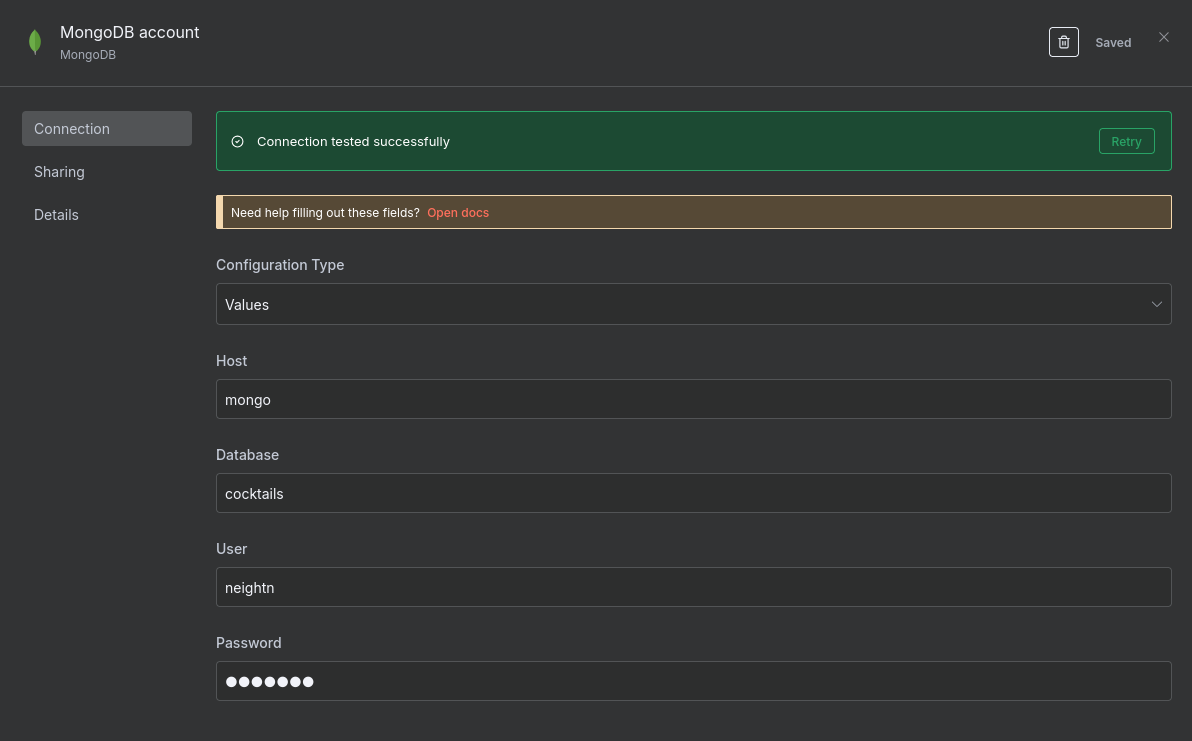
\includegraphics[width=0.95\textwidth]{images/n8n_mongo_creds.png}
    \end{center}
    \caption{n8n MongoDB Zugangsdaten}\label{fig:n8n_mongo_creds}
\end{figure}

Für die KI muss noch ein API Schlüssel von seinem OpenAI Benutzerkonto hinterlegt werden. Dazu wird
der zweite Zugangsdatum erstellt.

\begin{figure}
    \begin{center}
        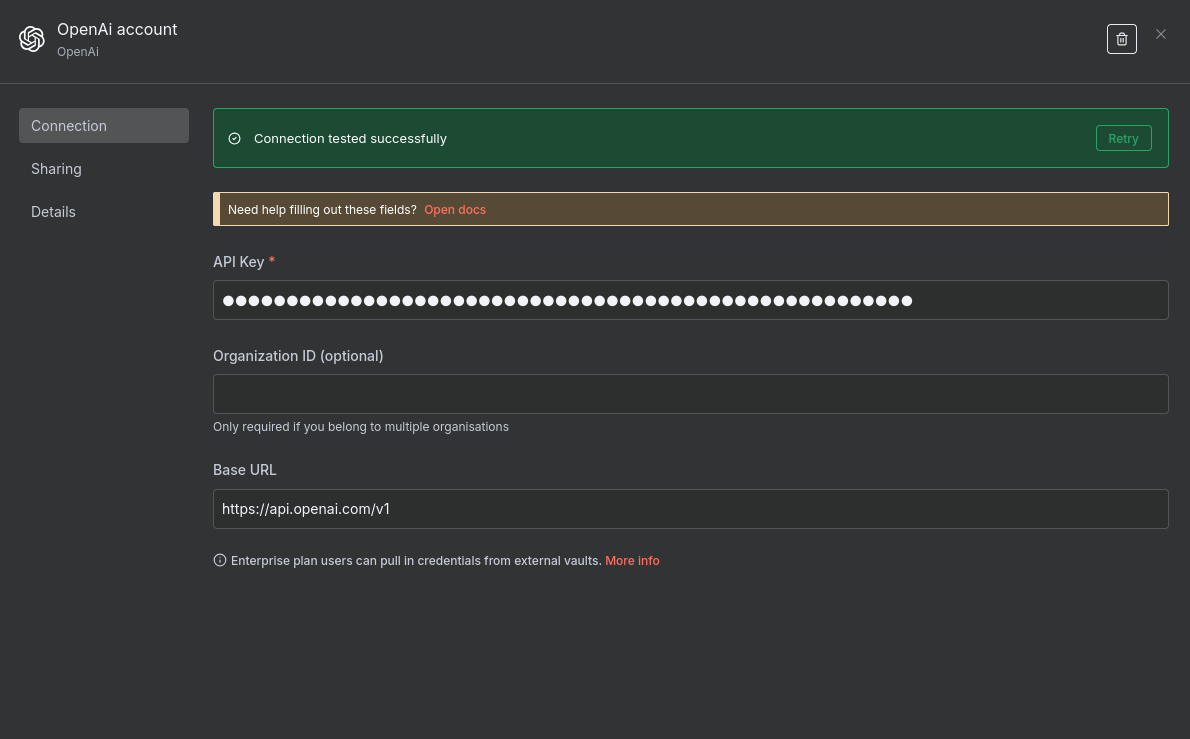
\includegraphics[width=0.95\textwidth]{images/n8n_openai_creds.png}
    \end{center}
    \caption{n8n OpenAI Zugangsdaten}\label{fig:n8n_openai_creds}
\end{figure}

Nachdem die beiden Zugangsdaten angelegt wurden, kann ein neuer Workflow erstellt werden. Im
Bearbeitungsmodus angekommen, befindet sich open rechts im Dreipunktemenü die Auswahl ein
vorhandenen Workflow von einer Datei zu importieren. Im ZIP-Archiv ist der Workflow unter dem Namen
\verb|Promillo.json| zu finden.

\begin{figure}
    \begin{center}
        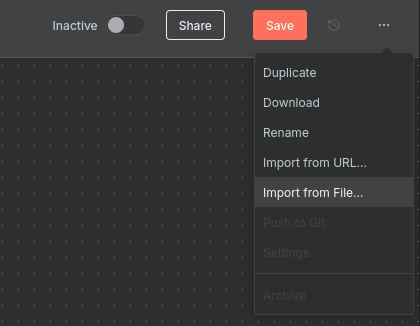
\includegraphics[width=0.95\textwidth]{images/n8n_import.png}
    \end{center}
    \caption{n8n Import Workflow}\label{fig:n8n_import}
\end{figure}

Die Nodes, die Zugangsdaten benötigen werden rot makiert, diese müssen mit Doppelklick einmal
geöffnet und in der obenren linken Ecke geschlossen werden. Die Zugangsdaten verwenden zwar den
standart Namen, werden von n8n aber mit eindeutigen IDs referenziert. Aufgrund des anlegens der
Zugangsdaten werden im Workflow nicht die richtigen IDs referenziert, durch das Öffnen und Schließen
werden die diese korriegiert.

Zum Schluss muss der Workflow in der open rechten Ecke gespeichert und aktiviert werden. Der
Workflow ist damit unter der eigenen Domaine mit dem Pfad \verb|/form/alcohol| erreichbar.

% section Cook (end)
